%------------------------------------------
% Este é o estilo/template de formatação de 
% TCC 2 no formato de artigo do DCC/UFRR.
% Este documento utiliza como base o modelo
% de formatação da SBC (Sociedade Brasileira
% de Computação). Disponivel em: 
% https://www.sbc.org.br/wp-content/uploads/2024/07/modelosparapublicaodeartigos.zip
%------------------------------------------

\documentclass[12pt]{article}

% --------------------------------------
% Pacotes utilizados 
% --------------------------------------
\usepackage{estilo/sbc-template}
\usepackage{tikz}
\usepackage{transparent}
\usepackage{graphicx,url}
\usepackage[utf8]{inputenc}
\usepackage[brazil]{babel}
\usepackage{todonotes}
\usepackage{fancyhdr}
\usepackage{multirow}
\usepackage{scalefnt}
\usepackage{float}
\usepackage{datetime}
\usepackage{ifthen}
\usepackage[alf]{abntex2cite} 
\usepackage{listings}
\usepackage{subcaption}
\usepackage{bigstrut}
\usepackage{array}


% --------------------------------------
% Configurações de formatação de código
% --------------------------------------
\lstset
{ %Formatting for code
    language=C,
    basicstyle=\footnotesize,
    numbers=left,
    stepnumber=1,
    frame = single,
    showstringspaces=false,
    tabsize=2,
    breaklines=true,
    xleftmargin=10pt,
    breakatwhitespace=false,
    extendedchars=true,
    literate={á}{{\'a}}1 
             {ã}{{\~a}}1
             {é}{{\'e}}1
             {í}{{\'i}}1
             {õ}{{\~o}}1
             {ç}{{\c{c}}}1,
}


% --------------------------------------
% Definições de formatação
% Númeração das páginas
% --------------------------------------
\pagestyle{fancy}
\fancyhf{}
\fancyhead[R]{\thepage}
\renewcommand{\headrulewidth}{0pt}


\sloppy

% --------------------------------------
% Definições de informações do TCC
% --------------------------------------
\title{TÍTULO DO TRABALHO}

\author{NOME DO DISCENTE}

\orientador{Prof. Título. Nome Completo}
% Caso não tenha coorientador, deixar o campo vazio.
\coorientador{}
% Caso tenha coorientador, descomentar linha abaixo.
%\coorientador{Prof. Título. Nome Completo}

\address{
  Curso de Bacharelado em Ciência da Computação\\ 
  Departamento de Ciência da Computação\\ 
  Universidade Federal de Roraima (UFRR)\\ 
  Boa Vista -- RR -- Brasil  
  \email{\{aluno\}@ufrr.br}
}

% Caso não tenha agradecimentos, deixar o campo vazio.
\agradecimento{
  \todo[inline]{É opcional, mas é comum que se escreva esta seção de modo a reconhecer todos que contribuíram de modo relevante com a elaboração do TCC, sejam pessoas ou organizações. Exemplo: A todos os professores do curso que colaboraram e construíram bases sólidas no meu desenvolvimento e aprendizagem para o crescimento profissional. Seus nomes são inesquecíveis e por isso, dedico-lhes minha profunda admiração e respeito.}
}
% --------------------------------------


% --------------------------------------
% Início do documento
% --------------------------------------
\begin{document} 

% Não é necessário alterar
% Capa personalizada para UFRR
\begin{titlepage}
    \begin{tikzpicture}[remember picture,overlay]
        \node[opacity=0.1,inner sep=0pt] at (current page.center){
            
\includegraphics[width=0.9\paperwidth]{estilo/dcc-logo.png}
        };
    \end{tikzpicture} 

    \begin{center}
        % Imagem no topo (troque o nome do arquivo para o correto)
        
\includegraphics[width=0.3\textwidth]{estilo/ufrr-logo.png} \\[2cm]

        % Instituição
        {\large
        UNIVERSIDADE FEDERAL DE RORAIMA\\
        CENTRO DE CIÊNCIAS E TECNOLOGIA\\
        DEPARTAMENTO DE CIÊNCIA DA COMPUTAÇÃO\\
        CURSO DE BACHARELADO EM CIÊNCIA DA COMPUTAÇÃO\\[3cm]
        }

        % Nome do aluno
        {\bfseries\Large Nome do Aluno}\\[1.5cm]

        % Título do trabalho
        {\bfseries\LARGE Título do Trabalho}\\[3.5cm]

        % Data
        {\large Boa Vista - RR\\
        Maio de 2025}
    \end{center}
\end{titlepage}

% Folha de rosto
%\newpage
\begin{titlepage}
    \begin{tikzpicture}[remember picture,overlay]
        \node[opacity=0.1,inner sep=0pt] at (current page.center){
            
\includegraphics[width=0.9\paperwidth]{estilo/dcc-logo.png}
        };
    \end{tikzpicture}
    \begin{center}
        % Título em negrito no topo
        {\bfseries\LARGE 
            \makeatletter
            \@title
            \makeatother
        }\\[4cm]

        % Nome do discente
        {\Large 
            \makeatletter
            \@author
            \makeatother
        }\\[4cm]

        % Texto com recuo à direita
        \begin{flushright}
            \parbox{9cm}{\setlength{\parindent}{0pt}
            Trabalho de Conclusão de Curso apresentado ao curso de Bacharelado em Ciência da Computação do Departamento de Ciência da Computação da Universidade Federal de Roraima, em cumprimento às exigências legais como requisito parcial à obtenção do título Bacharel em Ciência da Computação.
            }
        \end{flushright}

        \begin{flushright}
            \parbox{9cm}{\setlength{\parindent}{0pt}
            \textbf{Orientador:} Prof. Título. Nome Completo.
            }
        \end{flushright}

        \begin{flushright}
            \parbox{9cm}{\setlength{\parindent}{0pt}
            \textbf{Coorientador:} Prof. Título. Nome Completo.
            }
        \end{flushright}

        \vfill

        % Data ao final da página
        {\large Boa Vista - RR\\
        \today}
    \end{center}
\end{titlepage}

\ifagradecimentodefined{
  % Agradecimentos
% Este arquivo contém o conteúdo da página de agradecimentos do TCC.
%\newpage
\begin{titlepage}
    \begin{tikzpicture}[remember picture,overlay]
        \node[opacity=0.1,inner sep=0pt] at (current page.center){
            
\includegraphics[width=0.9\paperwidth]{estilo/dcc-logo.png}
        };
    \end{tikzpicture}
    \begin{center}
        % Título em negrito no topo
        {\bfseries\LARGE AGRADECIMENTOS}\\[4cm]

        % Texto de Agradecimentos
        {\bfseries\Large \todo[inline]{É opcional, mas é comum que se escreva esta seção de modo a reconhecer todos que contribuíram de modo relevante com a elaboração do TCC, sejam pessoas ou organizações. Exemplo: A todos os professores do curso que colaboraram e construíram bases sólidas no meu desenvolvimento e aprendizagem para o crescimento profissional. Seus nomes são inesquecíveis e por isso, dedico-lhes minha profunda admiração e respeito.}}

        

        \vfill

        % Data ao final da página
        {\large Boa Vista - RR\\
        \today}
    \end{center}
\end{titlepage}

}

% --------------------------------------
% Sumário
% --------------------------------------
\renewcommand{\contentsname}{\centering \bfseries SUMÁRIO}
\tableofcontents
\thispagestyle{empty}

\clearpage
\pagenumbering{arabic}
\maketitle

% --------------------------------------
% Resumo em português
% --------------------------------------
\begin{resumo} 
  \textcolor{red}{Comece com uma sentença apresentando o objetivo do estudo. Depois descreva o método. Passe para uma breve descrição de resultados, indicando, então, a conclusão do seu estudo. Finalize com uma frase que pode, por exemplo, convidar a comunidade científica para realizar mais estudos semelhantes ao seu ou que indique a contribuição do seu trabalho. O seu resumo deve ter, no máximo, 150 palavras ou 10 linhas. O mesmo vale para o abstract. Importante: em um resumo, tipicamente, não fazemos citações. Além disso, não se deve inserir fórmulas, equações, diagramas ou símbolos.}
\end{resumo}


% --------------------------------------
% Resumo em inglês
% --------------------------------------
\begin{abstract}
  \textcolor{red}{Dica para a produção de um resumo em inglês: traduza o texto em português com a ajuda do Google Tradutor. Depois use uma versão gratuita do Grammarly para avaliar a qualidade do texto. Aceite as sugestões desse software.}
\end{abstract}


% --------------------------------------
% Keywords do artigo
% --------------------------------------
\keywords{Word 1, Word 2, Word 3}


%--------------------------------------
% Seções do artigo
%--------------------------------------
\section{Introdução}
\label{sec:introducao}

\todo[inline]{\textbf{NOTA}: O texto aqui apresentado é apenas a informação sobre algumas regras, para o escrita do seu trabalho, o texto abaixo DEVE SER REMOVIDO.}

\textcolor{red}{A função da introdução é informar ao leitor o tema da pesquisa, destacar a sua relevância científica e/ou social, sendo finalizada com a descrição de como o TCC está organizado, ou seja, como está subdividido. É importante ressaltar que a introdução apresenta a visão geral do TCC. Ela precisa ser sedutora, de forma a mobilizar o leitor para seguir com a leitura. Apesar de ser o primeiro capítulo do trabalho, normalmente é o último a ser feito. O motivo é que só apresentamos aquilo que já escrevemos.}

\textcolor{red}{1) Comece com uma sentença descrevendo qual é o tema da sua pesquisa, já podendo indicar o que você pretende investigar. 2) Na sequência, você pode dar uma ideia muito geral do que tem sido investigado nesse tema e já passar para a apresentação dos motivos para a realização da pesquisa. Alternativamente, pode já começar pela motivação. Motivos são argumentos, isto é, justificativas que indicam por qual motivo a pesquisa foi realizada. Argumente, preferencialmente, com base em dados, números, de pesquisa por qual motivo esse tema é relevante para a ciência e/ou para a sociedade. O ideal seria ter de dois a três argumentos para justificar a importância da sua pesquisa. Use citações para sustentar os argumentos. Os seus argumentos também podem mostrar a relevância do tema a partir das implicações que ele possui para a sociedade.}

\textcolor{red}{3) Você deve, então, explicitar o que irá estudar dentro do seu tema, o que significa explicitar o seu problema de pesquisa. O problema pode ser apresentado de duas formas: como objetivo (verbo no infinitivo + complemento) ou como pergunta. No caso do TCC do DCC, vamos mesclar as duas estratégias, apresentando o objetivo geral do estudo e perguntas de pesquisa que, se respondidas, atendem ao objetivo geral.
[4) Finalize a introdução com a descrição das seções que compõem o seu trabalho.}

\textcolor{red}{Atenção com relação à estrutura explicada. De modo simples, ela propõe que você responda três perguntas, sendo uma resposta por parágrafo: 1) Qual é o tema da pesquisa e o que você irá estudar dentro dessa temática? 2) Quais os motivos que justificam o que você pretende estudar? 3) Como o seu TCC está organizado?}

\todo[inline]{\textbf{NOTA}: Qual o problema que você está tentando resolver através do trabalho? Quais as restrições de projeto envolvidas?}

O problema considerado neste trabalho é expresso na seguinte questão:

\todo[inline]{A pergunta de pesquisa precisa ser respondida para que o objetivo geral possa ser alcançado. Pensando nisso, elabore a sua questão. O seu principal compromisso na pesquisa é conseguir essa resposta. Você pode ter uma só pergunta ou mais. Relembrando: você precisará responder essas perguntas, portanto é razoável não escrever qualquer questão.}

O objetivo deste estudo é 
\todo[inline]{Preencher com texto iniciando com um verbo no infinitivo seguido de complemento. Escolha um dos seguintes verbos e complementos: “Conduzir revisão de literatura sobre…”, “Caracterizar a variável…”, “Descrever a variável…”, “Desenvolver sistema/aplicativo/aplicação/script…”, “Investigar validade…”, “Testar validade do modelo…”, “Testar a relação de associação entre as variáveis A e B”, “Testar a relação de determinação entre as variáveis A e B” etc.}

Visando contribuir com $\dots$, o contexto deste trabalho
está situado no uso de metodologias e técnicas de $\dots$
\todo[inline]{Você deve descrever a situação ou o contexto geral referente ao assunto em questão, devem constar informações atualizadas
visando a proporcionar maior consistência ao trabalho. Adicionalmente, uma breve descrição da solução proposta.}

\textbf{Organização do Trabalho.} As demais seções restantes são organizados da seguinte forma:
% 
Nos \textbf{Fundamentos Teóricos}, são apresentados os conceitos abordados neste trabalho, especificamente: \textcolor{red}{XXX, YYY, e ZZZ.}
%
Nos \textbf{Trabalhos Correlatos}, são analisados os trabalhos correlatos a solução proposta.
%
Na \textbf{Método da Solução Proposta}, é descrito as etapas de execução do método da solução proposta para \textcolor{red}{XXXX}.
%
No \textbf{Planejamento para Avaliação Experimental}, é apresentado o planejamento e projeto para execução da avaliação da solução proposta.
%
E por fim nas \textbf{Considerações Parciais}, apresenta-se as considerações parciais e análise das atividades já desenvolvidas.
\section{Fundamentos Teóricos}
\label{sec:fundamentos}

\todo[inline]{Aqui você vai selecionar os principais termos técnicos que precisam ser esclarecidos para que o leitor compreenda o seu trabalho e, ainda, vai explicar a teoria que está adotando. Use referências clássicas, mas também referências dos últimos cinco anos. Explique apenas os termos cruciais para o seu trabalho. Procure ser tão conciso quanto possível nesta seção. Não use citações literais. Não use citações de citações.}


\subsection{Fundamentos 1}
\label{sec:fundamentos1}
\todo[inline]{Segue \textbf{um exemplo} de apresentação de código na linguagem de programação C que pode ser utilizado na apresentação de conceitos.}

\begin{figure}[thp]	
    \centering
    \begin{subfigure}{0.4\textwidth}
    \centering
    \begin{lstlisting}[language=C]       
double custo(double entrada)
{
  if (entrada < 0) 
  {
    return -1;
  }
  if ((entrada * 1.5) <= 0)) 
  {
    return -1;
  }
  if(entrada > 50) 
  {
    return 1.25*entrada;
  }
  return 1.5*entrada;
}
	\end{lstlisting}
    \caption{Código C}
  \end{subfigure}%    
  \begin{subfigure}{.05\textwidth}
    \hfill
  \end{subfigure}%    
  \begin{subfigure}{.4\textwidth}
    \centering
\begin{lstlisting}[language=C]   
TEST_CASE_1()
{
  double result;
  result = custo(0.49)
  assert(result == 0.735);
}
TEST_CASE_2()
{
  double result;
  result = custo(51)
  assert(result == 63.75);
}
\end{lstlisting}
  \caption{Código de Teste}
  \end{subfigure}%
  \caption{\label{fig:program_test} Exemplo de código}
\end{figure}


\subsection{Fundamentos 2}
\label{sec:fundamentos2}

\todo[inline]{Segue um exemplo de uso de figura}

A Figura~\ref{fig_grafico} apresenta uma imagem.

\begin{figure}[h!]    
	\begin{center}
	    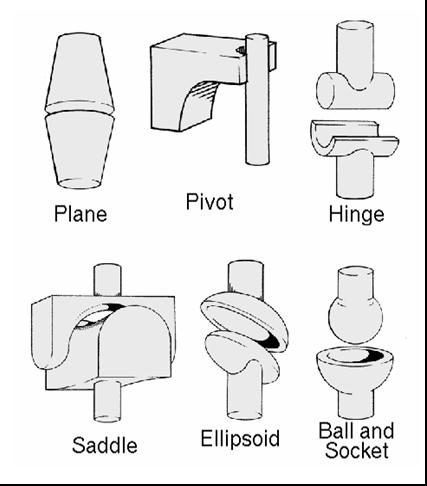
\includegraphics[scale=0.5]{imagens/fig2.jpg}
	\end{center}
    \caption{\label{fig_grafico}Descrição da iamgem.}
\end{figure}

\subsection{Fundamentos 3}
\label{sec:fundamentos3}

\todo[inline]{Segue um exemplo de uso referências.}

Segundo \citeonline{knuth:84}, tem-se que $\dots$ \cite{boulic:91} e \cite{smith:99}.
%------------------------------------------
% Trabalho Relacionados
%------------------------------------------
\section{Trabalhos Relacionados}
\label{sec:trabalhos-re}


\todo[inline]{Nesta parte faz-se a revisão de literatura sobre o assunto, resumindo-se os resultados de estudos feitos por outros autores, cujas obras citadas e consultadas devem constar nas referências.}

\textcolor{red}{A função desta seção é demonstrar o conhecimento já existente na ciência. O que faltar de conhecimento é lacuna e, portanto, novidade que você pode explorar, tomando, então, como seu problema de pesquisa. Deve conter, no mínimo, três pesquisas em formato de artigo científico, preferencialmente, dos últimos cinco anos. Você poderá obter esses estudos por indicação do orientador ou, por exemplo, no Google Acadêmico.}

\textcolor{red}{As pesquisas que você irá buscar para compor esta seção são aquelas semelhantes à sua, ou seja, que investigam o mesmo tema e que atacam problemas de pesquisa nos quais você está interessado em estudar.}

\textcolor{red}{A descrição de um estudo deve ocupar, idealmente, apenas um parágrafo. Como regra geral, um parágrafo pode ter até 20 linhas, mas tente trabalhar com o máximo de 12 ou 16. No máximo, a sua descrição de um estudo deve ocupar dois parágrafos, não mais que isso.}

\textcolor{red}{As descrições de estudos devem ser conectadas entre si por meio do texto. Ou seja, você pode afirmar que Santos (2022) investigou X e conclui Y, sugerindo como trabalho futuro Z. Aí, no parágrafo seguinte, você pode dizer que Silva (2022), baseado em Santos (2022), conduziu estudo para investigar Z. Note, portanto, que os estudos foram, de algum modo, conectados no seu texto.}

\textcolor{red}{Como regra geral, a descrição de um estudo deve seguir o seguinte formato, que você pode adaptar: “Silva e Santos (2022) conduziram estudo cujo objetivo foi {Preencher com o verbo no infinitivo mais complemento adotado por Silva e Santos}. Para atingir esse objetivo, adotaram o seguinte método: {Preencher com uma breve descrição do método do estudo}. Os pesquisadores verificaram que {Preencher com os principais dados}. A partir desses dados, concluíram que {Preencher com a resposta à principal pergunta de pesquisa}. Esse estudo teve como principais limitações: {Preencher com uma breve síntese}”.}

\textcolor{red}{O parágrafo final desta seção pode explicitar a correlação entre as pesquisas descritas e, então, explicitar de modo inequívoco a lacuna na literatura que justifica o problema de pesquisa que, na seção seguinte, será apresentado.}

\todo[inline]{Deve-se apresentar uma visão geral e comparativa dos trabalhos apresentados, bem como, cada trabalho apresentado pode contribuir com o seu trabalho. Sugere-se também apresentar uma tabela comparativa entre os trabalhos apresentados. Abaixo segue um exemplo:}

A seguir analisamos as técnicas (ver Tabela~\ref{Table:TechByPapers}) 
adotadas para a geração das invariantes de programa nos trabalhos apresentados anteriormente. Vale ressaltar que as técnicas identificadas foram:

\begin{itemize}
    \item \textbf{Análise de Predicados}. Analisando os métodos baseadas na análise de predicado, podemos observar que a análise de predicado fornece um apoio significativo na análise do programa para inferir propriedades sobre o comportamento do programa;
    %
    \item \textbf{Interpretação Abstratata}. É uma teoria da aproximação da semântica de linguagens de programação cuja aplicação principal é a análise estática;
    %
    \item \textbf{Lógica de Mill}. A lógica de Mill é adotada para caracterizar laços por meio de uma função que define o seu espaço de estados.
    %
    \item \textbf{\textit{Templates}}. Analisando as publicações, notamos que a adoção de \textit{templates} é importante para fornecer um suporte para guiar a inferência de invariantes de programas.
\end{itemize}{}

%\multicolumn{number cols}{align}{text} % align: l,c,r
%\multirow{number rows}{width}{text}
\begin{table}[htbp]  
  \centering  
  \scalefont{0.9}  
  \begin{tabular}{|c|c|c|c|c|}
    \hline
    % header
    % row 1 and 2
    \multicolumn{1}{|c|}{\multirow{2}{*}{\textbf{Artigos}}} & 
    % row 1
    \multicolumn{4}{c|}{\textbf{Técnicas}} \bigstrut\\
    \cline{2-5} &
    % row 2
    \textbf{Predicados} & \textbf{Int. Abstrata} & \textbf{Log. Mill} & \textbf{\textit{Templates}} \bigstrut\\
    \hline
    % body table - row 3
    Trabalho 1 & X &  &  &  \bigstrut\\
    \hline
    % body table - row 4
    Trabalho 2 &  & X & X &  \bigstrut\\
    \hline
    % body table - row 5
    Trabalho 3 & X & X &  & X \bigstrut\\
    \hline
    % body table - row 6
    Trabalho 4 & X & X &  & X \bigstrut\\
    \hline
  \end{tabular}  
  \caption{Classificação dos artigos por técnicas.}
  \label{Table:TechByPapers}
\end{table}%

%--------------------------------------
% Solução Proposta
%--------------------------------------
\section{Solução Proposta}
\label{sec:solucao-proposta}


\todo[inline]{\textbf{NOTA}: Deve-se apresentar a visão geral da solução proposta, nesta seção você deve apresentar metodologia do trabalho ou procedimentos metodológicos – deve constar o instrumental, os métodos e as técnicas aplicados para a elaboração do trabalho.}


%--------------------------------------
% Arquitetura
%--------------------------------------
\subsection{Arquitetura}

\todo[inline]{\textbf{NOTA}: Deve-se apresentar uma visão geral da solução proposta, exemplo, usando uma Big Picture. Abaixo segue um \textbf{exemplo}.} 

A Figura~\ref{fig_bigpicture} apresenta uma visão geral da solução proposta que visa o desenvolvimento e análise de uma sistema de irrigação usando tecnologias de IoT.

\begin{figure}[h!]    
	\begin{center}
	    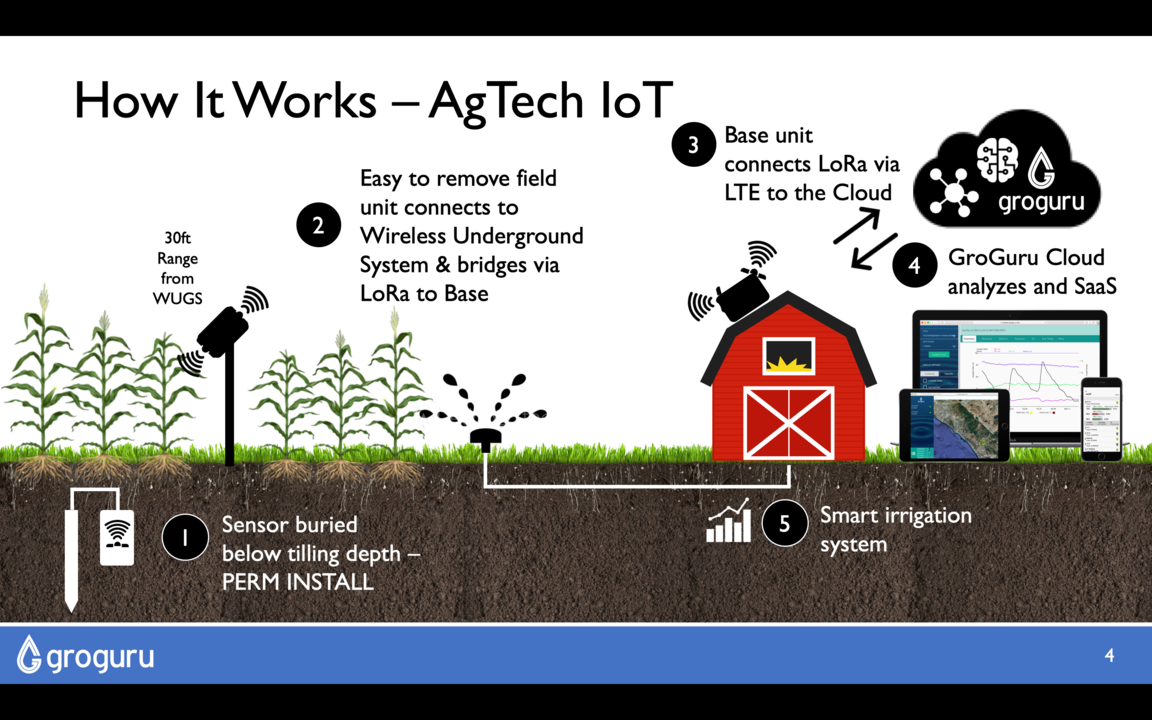
\includegraphics[scale=0.3]{imagens/bigpicture.png}
	\end{center}
	\caption{\label{fig_bigpicture}Como funciona o sistema de irrigação.}
\end{figure}

\todo[inline]{\textbf{NOTA}: Nesta seção, também deve-se apresentar o fluxo da sua solução, ou seja, um diagrama contendo os artefatos de entrada e saída para cada etapa da solução proposta. Um modelo de digrama que pode ser utilizado é o BPMN (http://www.bpmn.org). Abaixo segue um \textbf{exemplo}.}

A Figura~\ref{fig_digflow} apresenta o fluxo de execução da solução proposta contendo suas respectivas entradas e artefatos gerados no modelo BPMN.

\begin{figure}[h!]	
	\begin{center}
	    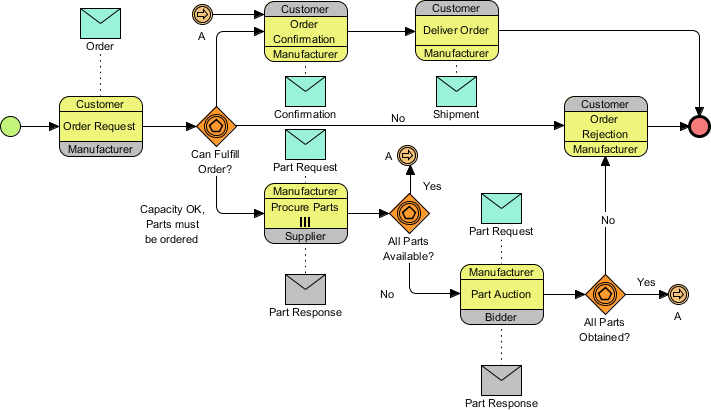
\includegraphics[scale=0.7]{imagens/34-final-business-process-diagram.png}
	\end{center}
    \caption{\label{fig_digflow}Diagram de fluxo no modelo BPMN.}
\end{figure}


%--------------------------------------
% Modelagem e Análise
%--------------------------------------
\subsection{Modelagem e Análise}
\label{sec:modelagem-analise}

\todo[inline]{Nesta subseção, apresenta-se um panorama da arquitetura da solução, destacando os principais componentes, entidades e interações. Deve-se adotar pelo menos um tipo de modelagem.}

\textcolor{red}{Exemplo: A solução proposta é composta por três módulos principais: (i) Interface do Usuário, (ii) Módulo de Processamento de Regras, e (iii) Gerenciador de Requisições. A comunicação entre os módulos é realizada por meio de eventos assíncronos. Para garantir a corretude das interações, utilizou-se modelagem formal com base em UML e Autômatos Finitos.}


\subsubsection{Modelagem com UML}

\textcolor{red}{Nesta parte, são apresentados os diagramas estruturais e comportamentais relevantes (e.g., casos de uso, atividades, estados, sequência, classes).}

\textcolor{red}{Exemplo:
%
A Figura 1 apresenta o Diagrama de Casos de Uso, onde é possível identificar os principais atores do sistema e suas interações com as funcionalidades.
A Figura 2 ilustra o Diagrama de Estados do componente Gerenciador de Requisições, evidenciando os estados "Inativo", "Aguardando Resposta" e "Erro de Timeout".}


\subsubsection{Modelagem com Autômatos Finitos}

\textcolor{red}{Aqui, são modelados formalmente os comportamentos dos módulos ou protocolos envolvidos, usando autômatos finitos determinísticos ou não determinísticos.}

\textcolor{red}{Exemplo:
%
O comportamento do módulo de autenticação foi modelado como um Autômato Finito Determinístico (AFD), conforme ilustrado na Figura 3.
O autômato possui os seguintes estados: q0 (esperando credenciais), q1 (verificação em andamento), q2 (acesso permitido), e q3 (acesso negado).
A transição de q0 para q1 ocorre ao receber um par usuário/senha; a transição para q2 ou q3 depende do resultado da verificação.}


\subsubsection{Modelagem com Redes de Petri}

\textcolor{red}{Utilize Redes de Petri para modelar e analisar aspectos concorrentes, sincronização e condições de deadlock.}

\textcolor{red}{Exemplo:
%
Para representar o processo de requisição e resposta entre cliente e servidor, modelamos o sistema utilizando uma Rede de Petri (Figura 4).
A rede inclui lugares como ClientePronto, RequisiçãoEnviada, ServidorOcupado e transições como EnviarRequisição, ProcessarRequisição, e ResponderCliente.
Foi verificada a ausência de deadlocks e a reentrância do sistema, assegurando que sempre será possível retornar ao estado inicial após uma interação completa.}


\subsubsection{Análise de Corretude}

\todo[inline]{\textbf{NOTA}: Aqui, discute-se os limites da modelagem, possíveis extensões e como os resultados reforçam a confiança na solução.}

\textcolor{red}{Apresente aqui os critérios de análise formal e os resultados obtidos com base nos modelos apresentados. Você pode usar ferramentas de verificação (ex: SPIN, TINA, NuSMV, UPPAAL) ou provas matemáticas.
%
Exemplo: A partir do modelo em autômatos, foi possível aplicar a verificação de propriedades de segurança e vivacidade.
Utilizando a ferramenta NuSMV, especificamos as propriedades desejadas em LTL (Linear Temporal Logic), como: $G(request -> F(response))$ - toda requisição será eventualmente respondida; $G \neg deadlock$ - ausência de deadlock em qualquer execução do sistema.
Todas as propriedades foram satisfatóriamente verificadas, confirmando a corretude formal da solução.}

\textcolor{red}{A modelagem revelou potenciais condições de corrida entre os módulos de log e autenticação, levando à introdução de um mecanismo adicional de controle de concorrência.
A utilização de três diferentes abordagens formais (UML, Autômatos, e Redes de Petri) permitiu uma análise multifacetada do sistema, contemplando tanto aspectos estruturais quanto comportamentais.}


\subsection{Ambiente de Desenvolvimento e Implementação da Solução}

\todo[inline]{\textbf{NOTA}: Deve-se apresentar as ferramentas já pesquisadas que serão adotadas na solução propostas, bem como, explicar como as ferramentas serão correlacionadas. \textbf{Importante}, mencionar o nome da ferramenta, versão e onde pode ser encontrada, segue um pequeno \textbf{exemplo} de uso.}

\textcolor{red}{Exemplo: A solução proposta será uma ferramenta de verificação de código implementada como um transformador de código escrita em C/C++ usando o \textit{framework} para compiladores LLVM~\footnote{https://llvm.org/} (v$6.0$). A solução utilizará como \textit{front-end} para programas escritos em C o Clang~\footnote{https://clang.llvm.org/} (v$6.0$ para gerar código LLVM-bitcode que será usado para a transformação de código. As ferramentas LibFuzzer (v$6.0$) e KLEE (v$2.0$) serão utilizadas para gerar entrada de testes para os códigos que serão analisados. Finalmente, o MetaSMT (v$4.rc2$) será usado como API para motores de solucionadores de satisfabilidade.}




%------------------------------------------
% Planejamento para Avaliação Experimental
%------------------------------------------
\section{Planejamento para Avaliação Experimental}
\label{sec:plan-experimentos}


\todo[inline]{\textbf{NOTA}: Deve-se adicionar um texto para introduzir o capitulo, segue um \textbf{exemplo}}

Esta seção descreve o planejamento para a execução da avaliação experimental da solução proposta, incluindo: o planejamento e projeto para a execução de um estudo experimental para avaliar o método proposto 
neste trabalho.


\subsection{Projeto da Avaliação Experimental}
\label{sub:experimento}

\todo[inline]{\textbf{NOTA}: Deve-se descrever o projeto para executar os testes para avaliar a solução proposta, incluindo o ambiente, elementos que serão utilizados, artefatos de entrada e saída, dados que serão coletados, e métricas para avaliação. Segue um \textbf{exemplo} abaixo.}

\textcolor{red}{Esta seção descreve o planeamento e concepção para a execução de um estudo empírico realizado com o objetivo de avaliar a solução proposta para \textcolor{red}{XXXXX}. O estudo será conduzido aplicando a solução proposta sobre \textit{benchmarks} públicos de programas em C. Os experimentos foram conduzidos em um computador Intel Xeon CPU E5, 2.60GHz, 115GB RAM com Linux 3.13.0 - 35-generic x86\_64.}

\todo[inline]{\textbf{NOTA}: Deve-se também apresentar como será executado a avaliação e qual o seu objetivo de cada ação na avaliação. Neste momento você deve considerar as formas de testar (cenários importante) e como coletar os dados para sua avaliação. Segue um \textbf{exemplo}. } 

\textcolor{red}{Esta avaliação empírica tem como objetivo analisar a capacidade do método proposto, sobre benchmarks públicos de programas em C, para contribuir com a verificação executada pelo software $X$. Desta forma, nesta avaliação, investiga-se as seguintes questões de pesquisa (QP):
%
\begin{itemize}
    \item[QP1]: As ferramentas para a geração de invariantes são capazes de suportar as diferentes estruturas da linguagem de programação C?
    %
    \item[QP2]: As abordagens propostas para geração de dados de teste contribuem para a geração de invariantes?
    %
    \item[QP3]: As invariantes geradas contribuem na verificação executada pelo ESBMC?
\end{itemize}}


\todo[inline]{\textbf{NOTA}: Deve-se também apresentar também as etapas da experimentação.}

%------------------------------------------
% Considerações Parciais
%------------------------------------------
\section{Considerações Parciais}
\label{sec:conclusao}


\todo[inline]{\textbf{NOTA}: Deve-se descrever as considerações parciais que formam a parte final (fechamento) do texto, sendo dito de forma resumida (1) o que foi desenvolvido no presente trabalho, (2) o que se espera após o desenvolvimento bem como as principais contribuições do trabalho, e (3) os desafios no desenvolvimento das próximas atividades do referido trabalho.}


%--------------------------------------
% Referências
%--------------------------------------
\bibliography{referencias}


%--------------------------------------
% Apêndice
%--------------------------------------
% Capa personalizada para UFRR
\begin{center}        
    \vspace*{\fill}
    {\Huge \textbf{APÊNDICES}}\\
    \vspace*{\fill}
\end{center}

%------------------------------------------
% Apendice 1
%------------------------------------------
\section{APÊNDICE 01 – CRONOGRAMA DE EXECUÇÃO DA PESQUISA}
\label{sec:apendice-1}


\todo[inline]{Você pode cadastrar mais atividades. Para cada atividade, indique com um X nas colunas à direita o tempo que você irá precisar para finalizá-la.}

\begin{table}[H]
    \centering
    \begin{tabular}{|l|c|c|c|c|}
        \hline
        \multirow{2}{7.5cm}{\textbf{Atividades}} & \multicolumn{4}{c|}{\textbf{Período de execução da pesquisa}} \\ \cline{2-5}
        & \textbf{Mês 01} & \textbf{Mês 02} & \textbf{Mês 03} & \textbf{Mês 04} \\ \hline
        Atividade 01 & X & X & X & X \\ \hline
        Atividade 02 &   &   &   &   \\ \hline
        Atividade 03 &   &   &   &   \\ \hline
    \end{tabular}
\caption{Cronograma de Execução da Pesquisa}
\end{table}
    


%--------------------------------------
% Anexos
%--------------------------------------
% Capa personalizada para UFRR
\begin{center}        
    \vspace*{\fill}
    {\Huge \textbf{ANEXOS}}\\
    \vspace*{\fill}
\end{center}

%------------------------------------------
% Título: Anexo 01 - Termo de responsabilidade do discente
%------------------------------------------
\section{ANEXO 01 - TERMO DE RESPONSABILIDADE DO DISCENTE}
\label{sec:anexo-1}

\todo[inline]{Anexos são recursos que outro pesquisador produziu e que você usou no seu trabalho. Todos os alunos possuem, necessariamente, 03 anexos.}


\section{ANEXO 02 - DECLARAÇÃO DE AUTORIA}

\begin{center}
    \fontsize{12}{15}\selectfont
    \vspace*{0.5cm}
    \textbf{DECLARAÇÃO DE AUTORIA}
    \vspace*{1cm}
\end{center}

\vspace*{\fill}

Eu, \textbf{Nome completo do discente} (código de matricula \textbf{0000000000}), autor da monografia/TCC (Trabalho de Conclusão de Curso) sob o título \textbf{ ... }, declaro que o trabalho em referência é de minha total autoria e de minha inteira responsabilidade o texto apresentado. Declaro, ainda, que as citações e paráfrases dos  autores estão indicadas com as respectivas obras e anos de publicação. Declaro, para os devidos fins que estou ciente:
\begin{itemize}\setlength\itemsep{.02em}
    \item  dos Artigos 297 a 299 do Código Penal, Decreto-Lei n. 2.848 de 7 de dezembro de 1940;
    %
    \item  da Lei n. 9.610, de 19 de fevereiro de 1998, sobre os Direitos Autorais; e
    %
    \item  que plágio consiste na reprodução de obra alheia e submissão da mesma como trabalho próprio ou na inclusão, em trabalho próprio, de ideias, textos, tabelas ou ilustrações (quadros, figuras, gráficos, fotografias, retratos, lâminas, desenhos, organogramas, fluxogramas, plantas, mapas e outros) transcritos de obras de terceiros sem a devida e correta citação da referência.
\end{itemize}

O corpo docente responsável pela avaliação deste trabalho poderá  não  aceitar o referido trabalho caso os pontos mencionados acima sejam descumpridos, por conseguinte, considerar-me reprovado.

\vspace*{\fill}

\begin{center}
    \rule{7cm}{0.4pt} \\
    \fontsize{12}{15}\selectfont Assinatura do acadêmico(a) \\ 
    Boa Vista - RR, data (por extenso).
\end{center}

\vfill


\end{document}
